\subsection{Quantum mechanics, part I}
This part offers a quick introduction to the necessary  quantum mechanics for readers whom are not familiar with the subject. The section contains nothing relevant for later parts of the thesis and can be safely skipped. For a more complete introduction I suggest chapter 1 of Sakurai.

\subsubsection{Dirac notation and quantum states}
A \textbf{quantum state} is a complex vector in a \textbf{Hilbert space}, a complete space with inner product induced metric, with finite or infinite dimension depending on characteristics of the system it represents. A quantum state vector is represented by a so-called \textbf{ket}, which is written as $\ket{\psi}$. Kets follow the same rules as a standard vector, as in that they can be added to one another, multiplied by a scalars. The ket itself is just $\ket{}$, the content of the ket is just a label which (usually) give some sense of what the state represents. \\
An \textbf{operator} is a matrix that can act on a ket, often defined by a set of rules. Written as 
\begin{equation}
\hat{O}\cdot (\ket{\psi}) = \hat{O}\ket{\psi}
\end{equation}
Since operators are matrices and kets are vectors, the existence of \textbf{eigenkets} are analogous eigenvectors. A common example of this is the time-independent Schrödinger equation
\begin{equation}
\hat{H}\ket{\psi} = E \ket{\psi}
\end{equation}
Where $\hat{H}$ is the Hamiltonian operator, and $E$ is the energy of the quantum state $\ket{\psi}$. In this case $\ket{\psi}$ is an eigenstate to the Hamiltonian.





\subsection{Lambda system}
A traditional $\Lambda$-system is a quantum mechanical system with two decoupled 'ground states' and one 'excited state' coupled to both ground states. Such a state with two ground state could realize a qubit by letting the ground state act as $\ket{0}$ and $\ket{1}$.

\begin{figure}[H]
    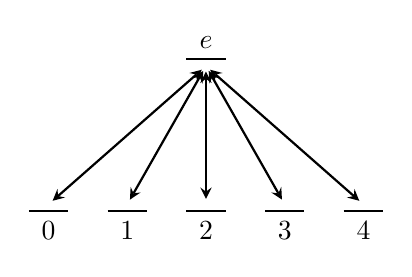
\begin{tikzpicture}[
      scale=0.5,
      level/.style={thick},
      virtual/.style={thick,densely dashed},
      trans/.style={thick,<->,shorten >=2pt,shorten <=2pt,>=stealth},
      classical/.style={thin,double,<->,shorten >=4pt,shorten <=4pt,>=stealth}]
      
    % Draw the energy levels.
    \draw[level] (6cm,0em) -- (7cm,0em) node[midway,above] {$\ket{e}$};
    \draw[level] (2cm,-11em) -- (3cm,-11em) node[midway,below] {$\ket{0}$};
    \draw[level] (4cm,-11em) -- (5cm,-11em) node[midway,below] {$\ket{1}$};
    \draw[level] (6cm,-11em) -- (7cm,-11em) node[midway,below] {$\ket{2}$};
    \draw[level] (8cm,-11em) -- (9cm,-11em) node[midway,below] {$\ket{3}$};
    \draw[level] (10cm,-11em) -- (11cm,-11em) node[midway,below] {$\ket{4}$};
    % Draw the transitions.
    
    \draw[trans] (6.5cm,-0.5em) -- (2.5cm,-10.5em) node[midway,left] {};
    \draw[trans] (6.5cm,-0.5em) -- (4.5cm,-10.5em) node[midway,left] {};
    \draw[trans] (6.5cm,-0.5em) -- (6.5cm,-10.5em) node[midway,left] {};
    \draw[trans] (6.5cm,-0.5em) -- (8.5cm,-10.5em) node[midway,left] {};
    \draw[trans] (6.5cm,-0.5em) -- (10.5cm,-10.5em) node[midway,left] {};
    %\draw[trans] (1cm,-2em) -- (2.5cm,8em) node[midway,left] {\ome{1}};
    %\draw[trans] (3.5cm,8em) -- (5cm,-8em) node[midway,right] {\Om{2}};
    %\draw[classical] (4.5cm,-8em) -- (1.5cm,-5em) node[midway,below] {\Ga{}};
    \end{tikzpicture}
    
    \caption{test figure}
\end{figure}

alfa $=$ $\frac{\pi}{2}\sin^{2}(\frac{\pi t}{T})$

beta $=$ $\eta(1 - \cos( \frac{\pi}{2}\sin^{2}(\frac{\pi t}{T}) ))$

alfa' $=$ $\frac{\pi^2}{2T}\sin(\frac{2\pi t}{T})$

beta' $=$ $\frac{\eta\pi^2}{2T}\sin(\frac{2\pi t}{T})\sin(\frac{\pi}{2}\sin^{2}(\frac{\pi t}{T}))$

\begin{equation*}
\Omega(t) = 2( (\frac{\eta\pi^2}{2T}\sin(\frac{2\pi t}{T})\sin(\frac{\pi}{2}\sin^{2}(\frac{\pi t}{T})))\cot(\frac{\pi}{2}\sin^{2}(\frac{\pi t}{T}))\sin(\eta(1 - \cos( \frac{\pi}{2}\sin^{2}(\frac{\pi t}{T}) )))
\end{equation*}
\begin{equation*}
+ \eta(1 - \cos( \frac{\pi}{2}\sin^{2}(\frac{\pi t}{T}) ))\cos(\eta(1 - \cos( \frac{\pi}{2}\sin^{2}(\frac{\pi t}{T}) ))) )
\end{equation*}



\subsection{Coupled excited states}
Hamiltonian of a ''double'' tripod
\begin{equation}
H(t) = \sum^2_{i = 1} \sum^3_{j = 1} \omega_{ij} \ket{j}\bra{e_i} + \text{h.c}
\end{equation}

Find dark states $H(t)\ket{d} = 0\ket{d} $ on form $\ket{d} = \sum_{k = 1}^3 d_k \ket{k}$
Result

\begin{equation}
\begin{aligned} &
d_1 = \frac{1}{\omega^{*}_{11}} \left(\omega^{*}_{12}\omega^{*}_{23}  - \omega^{*}_{13}\omega^{*}_{22} \right)
\\ &
d_2 = \frac{\omega^{*}_{13}\omega^{*}_{21}}{\omega^{*}_{11}} - \omega^{*}_{23}
\\ &
d_3 = \omega^{*}_{22} - \frac{\omega^{*}_{12}\omega^{*}_{21}}{\omega^{*}_{11}}
\end{aligned}
\end{equation}

Bright state $\bra{b}\ket{d} = 0$ 

\begin{equation}
\begin{aligned} &
\ket{b_1} = \omega_{11}\ket{1} + \omega_{12}\ket{2} + \omega_{13}\ket{3}
\\ &
\ket{b_2} = \omega_{21}\ket{1} + \omega_{22}\ket{2} + \omega_{23}\ket{3}
\end{aligned}
\end{equation}
Check if $\bra{b_1}\ket{b_2} = 0$? Holds if $\omega_{11} = -\frac{1}{\omega^{*}_{21}}\left(\omega^{*}_{12}\omega_{22} + \omega_{13}\omega^{*}_{23} \right)$


\newpage
% This LaTeX was auto-generated from MATLAB code.
% To make changes, update the MATLAB code and republish this document.

\sloppy
\definecolor{lightgray}{gray}{0.5}
\setlength{\parindent}{0pt}

    
    \begin{verbatim}
clear all;
syms(sym('w', [2 3]));
syms(sym('d',[1 3]));

H = [0, 0, w1_1, w1_2, w1_3;
      0, 0, w2_1, w2_2, w2_3;
      conj(w1_1), conj(w2_1), 0, 0, 0;
      conj(w1_2), conj(w2_2), 0, 0, 0;
      conj(w1_3), conj(w2_3), 0, 0, 0];



  H_d = simplify(eig(H))
\end{verbatim}

        \color{lightgray} \begin{verbatim} 
H_d =
                                                                                                                                                                                                                                                                                                                                                                                                                                                                                                                                                                                                                                                                                                     0
 -(2^(1/2)*(abs(w1_1)^2 + abs(w1_2)^2 + abs(w1_3)^2 + abs(w2_1)^2 + abs(w2_2)^2 + abs(w2_3)^2 - (abs(w1_1)^4 + abs(w1_2)^4 + abs(w1_3)^4 + abs(w2_1)^4 + abs(w2_2)^4 + abs(w2_3)^4 + 2*abs(w1_1)^2*abs(w1_2)^2 + 2*abs(w1_1)^2*abs(w1_3)^2 + 2*abs(w1_2)^2*abs(w1_3)^2 + 2*abs(w1_1)^2*abs(w2_1)^2 - 2*abs(w1_1)^2*abs(w2_2)^2 - 2*abs(w1_2)^2*abs(w2_1)^2 - 2*abs(w1_1)^2*abs(w2_3)^2 + 2*abs(w1_2)^2*abs(w2_2)^2 - 2*abs(w1_3)^2*abs(w2_1)^2 - 2*abs(w1_2)^2*abs(w2_3)^2 - 2*abs(w1_3)^2*abs(w2_2)^2 + 2*abs(w1_3)^2*abs(w2_3)^2 + 2*abs(w2_1)^2*abs(w2_2)^2 + 2*abs(w2_1)^2*abs(w2_3)^2 + 2*abs(w2_2)^2*abs(w2_3)^2 + 4*w1_1*w2_2*conj(w1_2)*conj(w2_1) + 4*w1_2*w2_1*conj(w1_1)*conj(w2_2) + 4*w1_1*w2_3*conj(w1_3)*conj(w2_1) + 4*w1_3*w2_1*conj(w1_1)*conj(w2_3) + 4*w1_2*w2_3*conj(w1_3)*conj(w2_2) + 4*w1_3*w2_2*conj(w1_2)*conj(w2_3))^(1/2))^(1/2))/2
 
 -(2^(1/2)*(abs(w1_1)^2 + abs(w1_2)^2 + abs(w1_3)^2 + abs(w2_1)^2 + abs(w2_2)^2 + abs(w2_3)^2 + (abs(w1_1)^4 + abs(w1_2)^4 + abs(w1_3)^4 + abs(w2_1)^4 + abs(w2_2)^4 + abs(w2_3)^4 + 2*abs(w1_1)^2*abs(w1_2)^2 + 2*abs(w1_1)^2*abs(w1_3)^2 + 2*abs(w1_2)^2*abs(w1_3)^2 + 2*abs(w1_1)^2*abs(w2_1)^2 - 2*abs(w1_1)^2*abs(w2_2)^2 - 2*abs(w1_2)^2*abs(w2_1)^2 - 2*abs(w1_1)^2*abs(w2_3)^2 + 2*abs(w1_2)^2*abs(w2_2)^2 - 2*abs(w1_3)^2*abs(w2_1)^2 - 2*abs(w1_2)^2*abs(w2_3)^2 - 2*abs(w1_3)^2*abs(w2_2)^2 + 2*abs(w1_3)^2*abs(w2_3)^2 + 2*abs(w2_1)^2*abs(w2_2)^2 + 2*abs(w2_1)^2*abs(w2_3)^2 + 2*abs(w2_2)^2*abs(w2_3)^2 + 4*w1_1*w2_2*conj(w1_2)*conj(w2_1) + 4*w1_2*w2_1*conj(w1_1)*conj(w2_2) + 4*w1_1*w2_3*conj(w1_3)*conj(w2_1) + 4*w1_3*w2_1*conj(w1_1)*conj(w2_3) + 4*w1_2*w2_3*conj(w1_3)*conj(w2_2) + 4*w1_3*w2_2*conj(w1_2)*conj(w2_3))^(1/2))^(1/2))/2
 
  (2^(1/2)*(abs(w1_1)^2 + abs(w1_2)^2 + abs(w1_3)^2 + abs(w2_1)^2 + abs(w2_2)^2 + abs(w2_3)^2 - (abs(w1_1)^4 + abs(w1_2)^4 + abs(w1_3)^4 + abs(w2_1)^4 + abs(w2_2)^4 + abs(w2_3)^4 + 2*abs(w1_1)^2*abs(w1_2)^2 + 2*abs(w1_1)^2*abs(w1_3)^2 + 2*abs(w1_2)^2*abs(w1_3)^2 + 2*abs(w1_1)^2*abs(w2_1)^2 - 2*abs(w1_1)^2*abs(w2_2)^2 - 2*abs(w1_2)^2*abs(w2_1)^2 - 2*abs(w1_1)^2*abs(w2_3)^2 + 2*abs(w1_2)^2*abs(w2_2)^2 - 2*abs(w1_3)^2*abs(w2_1)^2 - 2*abs(w1_2)^2*abs(w2_3)^2 - 2*abs(w1_3)^2*abs(w2_2)^2 + 2*abs(w1_3)^2*abs(w2_3)^2 + 2*abs(w2_1)^2*abs(w2_2)^2 + 2*abs(w2_1)^2*abs(w2_3)^2 + 2*abs(w2_2)^2*abs(w2_3)^2 + 4*w1_1*w2_2*conj(w1_2)*conj(w2_1) + 4*w1_2*w2_1*conj(w1_1)*conj(w2_2) + 4*w1_1*w2_3*conj(w1_3)*conj(w2_1) + 4*w1_3*w2_1*conj(w1_1)*conj(w2_3) + 4*w1_2*w2_3*conj(w1_3)*conj(w2_2) + 4*w1_3*w2_2*conj(w1_2)*conj(w2_3))^(1/2))^(1/2))/2
  
  (2^(1/2)*(abs(w1_1)^2 + abs(w1_2)^2 + abs(w1_3)^2 + abs(w2_1)^2 + abs(w2_2)^2 + abs(w2_3)^2 + (abs(w1_1)^4 + abs(w1_2)^4 + abs(w1_3)^4 + abs(w2_1)^4 + abs(w2_2)^4 + abs(w2_3)^4 + 2*abs(w1_1)^2*abs(w1_2)^2 + 2*abs(w1_1)^2*abs(w1_3)^2 + 2*abs(w1_2)^2*abs(w1_3)^2 + 2*abs(w1_1)^2*abs(w2_1)^2 - 2*abs(w1_1)^2*abs(w2_2)^2 - 2*abs(w1_2)^2*abs(w2_1)^2 - 2*abs(w1_1)^2*abs(w2_3)^2 + 2*abs(w1_2)^2*abs(w2_2)^2 - 2*abs(w1_3)^2*abs(w2_1)^2 - 2*abs(w1_2)^2*abs(w2_3)^2 - 2*abs(w1_3)^2*abs(w2_2)^2 + 2*abs(w1_3)^2*abs(w2_3)^2 + 2*abs(w2_1)^2*abs(w2_2)^2 + 2*abs(w2_1)^2*abs(w2_3)^2 + 2*abs(w2_2)^2*abs(w2_3)^2 + 4*w1_1*w2_2*conj(w1_2)*conj(w2_1) + 4*w1_2*w2_1*conj(w1_1)*conj(w2_2) + 4*w1_1*w2_3*conj(w1_3)*conj(w2_1) + 4*w1_3*w2_1*conj(w1_1)*conj(w2_3) + 4*w1_2*w2_3*conj(w1_3)*conj(w2_2) + 4*w1_3*w2_2*conj(w1_2)*conj(w2_3))^(1/2))^(1/2))/2
 
\end{verbatim} \color{black}
    
Change basis, 
\begin{equation}
T = \begin{pmatrix}
1 & 0 & 0 & 0 & 0 \\
0 & 1 & 0 & 0 & 0  \\
0 & 0 & \omega_{11} & \omega_{21} & d_1  \\
0 & 0 & \omega_{12} & \omega_{22} & d_2  \\
0 & 0 & \omega_{13} & \omega_{23} & d_3  \\
\end{pmatrix}
\end{equation}

New hamiltonian in $\{\ket{e_1}, \ket{e_2}, \ket{b_1}, \ket{b_2}, \ket{d} \}$ is 
\begin{equation}
H_d(t) = T^\dagger H(t) T = \left(\sum_{j = 1}^2 \sum_{k = 1}^3 \left( \omega_{jk} \right)^2 \ket{b_j}\bra{e_j}\right) + \left[\omega_{11}\omega_{12} + \omega_{12}\omega_{22} + \omega_{13}\omega_{23} \right]\left(\ket{b_2}\bra{e_1} + \ket{b_1}\bra{e_2}\right)\; + \;\text{h.c} 
\end{equation} 
\note{Double check this calculation.}


Subspace is  $\{\ket{e_1}, \ket{e_2}, \ket{b_1}, \ket{b_2} \}$ since $\ket{d}$ is decoupled.\\
Simplify notation, $\Omega_j = \sum_{k = 1}^3 \omega_{jk}^2$ and $\Gamma = \omega_{11}\omega_{12} + \omega_{12}\omega_{22} + \omega_{13}\omega_{23}$ now Hamiltonian looks like 
\begin{equation}
H_d = \sum_{j = 1}^2 \Omega_j \ket{b_j}\bra{e_j} + \Gamma\left(\ket{b_2}\bra{e_1} + \ket{b_1}\bra{e_2} \right) + \; \text{h.c}
\end{equation}
\\
Now find a ''dark path'' $\ket{D(t)}$ such that $\bra{D(t)}H_d(t)\ket{D(t)} = 0$
\\ Set
\begin{equation}
 \ket{D} = a_1\ket{e_1} + a_2\ket{e_2} + c_1\ket{b_1} + c_2\ket{b_2}
\end{equation} 
Then 
\begin{equation}
H_d \ket{D} = \left(a_1\Omega_1 + a_2\Gamma \right)\ket{b_1} + \left(c_1 \Omega_1^{*} + c_2\Gamma^{*} \right)\ket{e_1} + \{1 \leftrightarrow 2 \}
\end{equation}

\begin{equation}
\bra{D}H_d\ket{D} = c_1^{*}\left(a_1\Omega_1 + a_2\Gamma\right) + a_1^{*}\left(c_1 \Omega_1^{*} + c_2\Gamma^{*} \right) + \{1 \leftrightarrow 2 \} = 0
\end{equation}
Written out, find $a_1,a_2,c_1,c_2$ such that
\begin{equation}
c_1^{*}\left(a_1\Omega_1 + a_2\Gamma\right) + c_2^{*}\left(a_2\Omega_2 + a_1\Gamma\right) + a_1^{*}\left(c_1 \Omega_1^{*} + c_2\Gamma^{*} \right) + a_2^{*}\left(c_2 \Omega_2^{*} + c_1\Gamma^{*} \right) = 0
\end{equation}

Vilka antaganden kan göras om $\Omega_j, \Gamma$?\\
Diagonalisera $H_d$? Räkna endast gemetrisk fas?





\end{document}


